\documentclass[10pt,pscyr,nonums]{hedlab}
\usepackage[russian]{babel}
\usepackage{hedmaths}
\usepackage{graphicx}
\graphicspath{{images/}, {plots/}}

\newgeometry{top=1.5cm, bottom=1.5cm, left=1cm, right=1cm}

\student{} \date{}
\labnum{502}
\labname{Изучение законов внешнего фотоэффекта}

\begin{document}
    \makeheader

    \emph{Цель работы:} практическое ознакомление с закономерностями внешнего
    фотоэффекта; экспериментальное определение работы выхода электрона из
    сурьмяно-цезиевого фотокатода, красной границы фотоэффекта, а также
    постоянной Планка.
    
    \emph{Используемые при расчетах формулы:}
    \( \omega = 2\pi c/\lambda; \ \hbar = eU_*/\omega_0; \ A_0 = \hbar\omega_0 \).

    \begin{figure}[h!]
        \center
        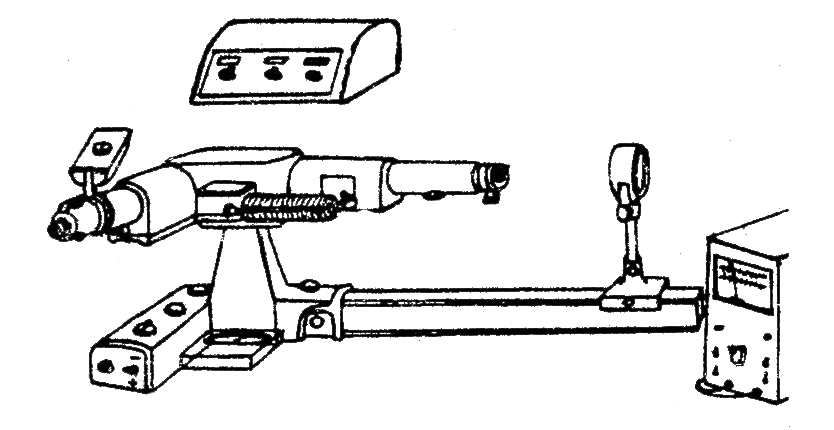
\includegraphics[width=.4\textwidth]{appearance} \hspace*{2em}
        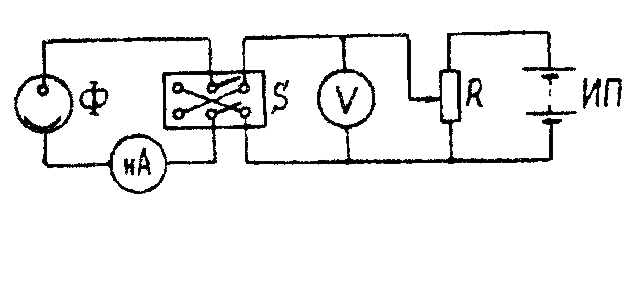
\includegraphics[width=.4\textwidth]{scheme} \\[.5em]
        \parbox{.4\textwidth}{\caption{Внешний вид установки}} \hspace*{2em}
        \parbox{.4\textwidth}{\caption{Схема подключения фотоэлемента}}
    \end{figure}
    \vspace*{-2em}
    
    \begin{table}[h!]
        \center \caption{Измерение запирающего напряжения}
        \begin{tabular}{|*{2}{C{.12}|}*{5}{C{.05}|}} \hline
            \multirow{2}{*}{Длина волны} &
                \multirow{2}{*}{Частота} &
                \multicolumn{5}{c|}{Задерживающее напряжение} \\ \cline{3-7}
            && \multicolumn{3}{c|}{\( U_\text{з} \)} &
                \multicolumn{2}{c|}{\( \midnum{U_\text{з}} \)} \\ \hline
            Нм & \( 10^{15}~\text{с}^{-1} \) &
                Дел & Дел & Дел & Дел & В \\ \hline
            &&&&&& \\ \hline
            &&&&&& \\ \hline
            &&&&&& \\ \hline
        \end{tabular}
    \end{table}
    
    \begin{table}[h!]
        \center \caption{Вольт-амперные характеристики фотокатода}
        \begin{tabular}{|C{.12}|*{7}{C{.05}|}} \hline
            Длина волны \( \lambda \),~нм &
                \( U \),~В & 0 & 0,6 &
                1,2 & 1,8 & 2,4 & 3,0 \\ \hline
            404,7 & \( I \),~нА &&&&&& \\ \hline
            435,6 & \( I \),~нА &&&&&& \\ \hline
            546,6 & \( I \),~нА &&&&&& \\ \hline
        \end{tabular}
    \end{table}
    
    \begin{table}[h!]
        \center \caption{Однократные измерения}
        \begin{tabular}{|*{6}{C{.12}|}} \hline
            \multirow{3}{*}{\( \omega_0 \), \( 10^{15}~\text{с}^{-1} \)} &
                \multirow{3}{*}{\( U_* \),~В} &
                \multicolumn{2}{c|}{\multirow{2}{*}{Работа выхода \( A_0 \)}} &
                Красная & Постоянная \\
            && \multicolumn{2}{c|}{} &
                граница & Планка \\ \cline{3-4}
            && \( 10^{-19} \)~Дж & эВ &
                \( \lambda_0 \),~нм &
                \( \hbar \),~Дж\(\cdot\)с \\ \hline
            &&&&& \\ \hline
        \end{tabular}
    \end{table}
    
    \pagebreak
    
    \subsection{Подсчет погрешности и окончательные результаты}
    \center
    \rule{.95\textwidth}{.5pt} \\ \rule{.95\textwidth}{.5pt}
    \rule{.95\textwidth}{.5pt} \\ \rule{.95\textwidth}{.5pt}
    \rule{.95\textwidth}{.5pt} \\ \rule{.95\textwidth}{.5pt}
    \rule{.95\textwidth}{.5pt} \\ \rule{.95\textwidth}{.5pt}
    \rule{.95\textwidth}{.5pt} \\ \rule{.95\textwidth}{.5pt} \\
    \vspace*{2em}
    
    \emph{Вывод:} \rule{.885\textwidth}{.5pt}
    \rule{.95\textwidth}{.5pt} \\ \rule{.95\textwidth}{.5pt}
    \rule{.95\textwidth}{.5pt}
\end{document}
